\section{Kriptanalisis dan Kriptologi}
\label{sec:kriptanalisis}

\textbf{Kriptanalisis} (\textit{cryptanalysis}) adalah ilmu dan seni memecahkan
cipherteks menjadi plainteks tanpa mengetahui kunci yang digunakan. Pelakunya
disebut kriptanalis. Kriptanalisis merupakan ``lawan'' kriptografi. Teknik ini
sudah ada sejak abad ke-9.

Kriptanalisis dikemukakan pertama kali oleh ilmuwan Arab pada abad ke-9 bernama
Abu Yusuf Yaqub Ibnu Ishaq Ibnu As-Sabbah Ibnu 'Omran Ibnu Ismail Al-Kindi, atau
Al-Kindi. Ia menulis buku berjudul \textit{Risalah fi Istikhraj al-Mu'amma}
(\textit{Manuscript for the Deciphering Cryptographic Messages}). Al-Kindi
menemukan keteraturan frekuensi perulangan huruf di dalam Al-Quran. Teknik itu
kemudian disebut \textbf{analisis frekuensi}, yaitu teknik memecahkan cipherteks
berdasarkan frekuensi kemunculan karakter. Gagasannya sederhana: pada bahasa
alami, huruf tidak muncul sama sering, dan pola itu tetap terbawa meskipun
identitas huruf telah disamarkan.

Sejarah kriptanalisis mencatat pemecahan Telegram Zimmermann, yang membawa
Amerika Serikat masuk ke Perang Dunia I. Pesan rahasia Menteri Luar Negeri
Jerman itu berisi tawaran aliansi kepada Meksiko dan berhasil dibaca pihak
Sekutu.

\textbf{Kriptologi} (\textit{cryptology}) adalah studi yang mencakup kriptografi
dan kriptanalisis. Hubungan keduanya tampak pada
Gambar~\ref{fig:kriptologi-cabang}: keduanya berdiri sejajar di bawah
kriptologi.

\begin{figure}[htbp]
    \centering
    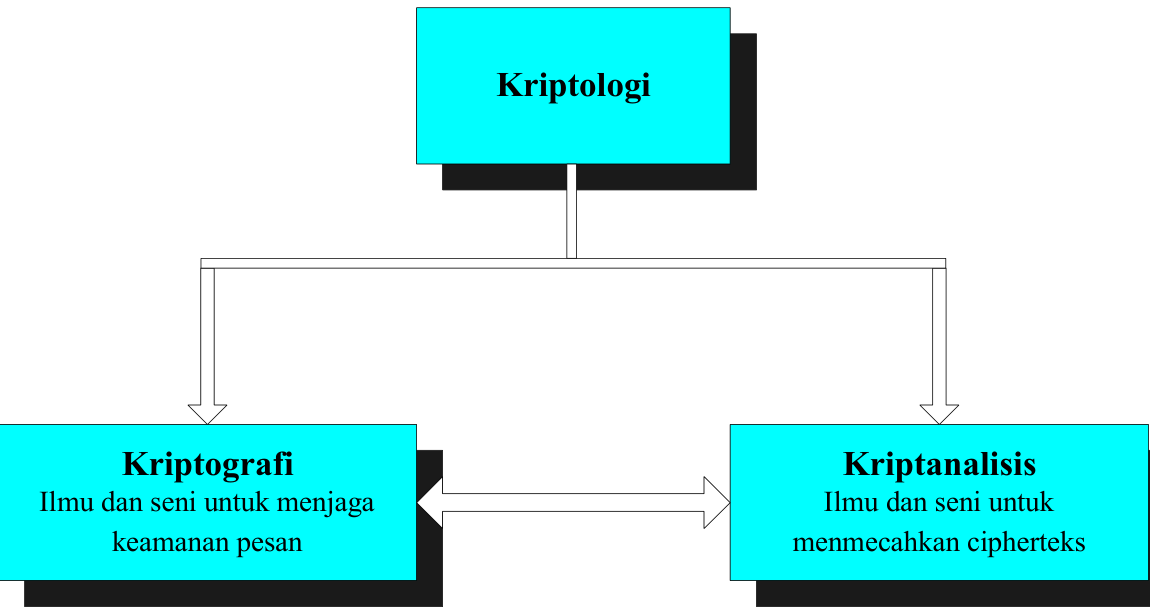
\includegraphics[width=0.62\linewidth, height=0.7\textheight, keepaspectratio]{figures/kriptologi-cabang.png}
    \caption{Kriptologi mencakup kriptografi yang merancang cara merahasiakan pesan dan kriptanalisis yang memecahkan cipherteks}
    \label{fig:kriptologi-cabang}
    \sumber{Munir, \textit{IF4020 Kriptografi}, ITB.}
\end{figure}
